% !TEX root = ../report.tex

\chapter{Final Discussions}
\label{sec:final_discussion}

This chapter provides some final discussions based on the results and experiences obtained from working with control-bounded ADC in general and the proposed Hadamard ADC architecture in particular. In this chapter, some discussions that did not fit naturally in the previous chapters are presented. There are also a lot of relevant topics that is beyond the scope of this thesis, and some of the limitations of the presented work is mentioned.

\section{Additional Features of the control-bounded ADCs}
\subsection{Shared Analog State Space}
It has been pointed out in section \ref{sec:advanced_DC} that there is a significant potential in utilizing the shared control system of the Hadamard ADC. A shared control enables a more effective distribution of the available control resources, and hence a tighter state bound and increased performance.

In the multi-channel Hadamard ADC, the different input channels also shares the analog state-space. If there are an unequal distribution of the signal energy between the different input channels, combining them through the Hadamard matrix will have an averaging effect. More precisely, if the input signal is more concentrated in one of the physical dimensions than in one of the Hadamard dimensions, the inputs to the first column of integrators (i.e. $x_0$-$x_3$ of fig \ref{fig:HCI_AS_01}) will have a more even distribution of energy than the input channels of the ADC. This effect could be utilized in terms of lowering the state bound or alternatively increasing the gain of the analog system, compared to the situation where each input channel is converted independently. Formally, the analog system could be scaled more towards $\E\left[ \norm{\utv}{2} \right]$, rather than $\E \left[ \norm{\utv}{\infty} \right]$, which would be required when each channel lies in a separate state-space.

This effect is illustrated in figure \ref{fig:signal_dimension}. The illustration is meant to give a simplified picture of the situation when a pulse is coming towards a receiver array, as a plane wave with a steep angle. The receiver array has two elements, and due to the angle of incident, the pulse reaches the two elements at different times. The signal from the two elements are denoted $u_0(t)$ and $u_1(t)$ respectively. Through the Hadamard matrix, the input signals are combined in an orthogonal way. The resulting normalized outputs signals, denoted $\tilde{u}_0(t)$ and $\tilde{u}_1(t)$, are illustrated at the right side of the Hadamard matrix.

The pictured situation is the ideal application for a Hadamard ADC. At any time instance, the signal energy lies almost entirely in one of the physical dimensions, i.e. $u_0(t)$ or $u_1(t)$. Hence, the energy becomes evenly distributed between the outputs $\tilde{u}_0(t)$ and $\tilde{u}_1(t)$. The magnitude of each output is reduced by a factor $\sqrt{2}$ relative to the input, but the effect is barely visible for the illustrated situation of two channels. For a larger system with hundreds or thousands of input channels, a scaling of $\sqrt{L}$ would be significant. As mentioned, this reduced signal strength could be utilized in terms of increased gain or tighter control bound. From equation (\ref{eq:analytic_snr_est}) we see that increasing the integrator gain, or lowering the state boundary, by a factor $\sqrt{L}$ would both give an SNR increasement proportional to $L$.
\begin{figure}[htbp]
    \centering
    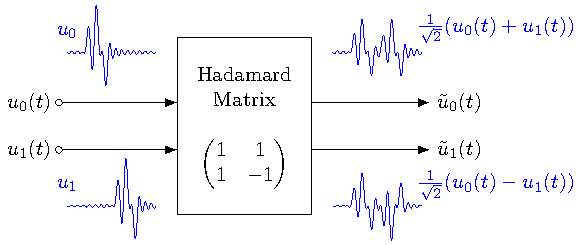
\includegraphics[width=\linewidth]{figures/05hadamard/signal_dimension.pdf}
    \caption{An illustration of a pulse arriving at two different receiver elements at different times. $\utv = \Tr{\left( u_0(t) , u_1(t) \right)}$ is the input signal and $\tilde{\bm{u}}(t) = \Tr{\left( \tilde{u}_0(t) , \tilde{u}_1(t) \right)}$ is the output signal of the Hadamard matrix.}
    \label{fig:signal_dimension}
\end{figure}


Figure \ref{fig:hadamard_dimension} pictures the opposite situation. In this case the pulse arrives at the two inputs almost simultaneously, and the signal energy lies almost entirely in the first Hadamard dimension. In consequence, almost all energy is concentrated at the first output of the Hadamard matrix, $\tilde{u}_0(t)$. The magnitude of $\tilde{u}_0(t)$ is therefore increased by $\sqrt{L}$ relative to the input, which would require a reduction in gain or state bound, and hence decreased SNR.
\begin{figure}[htbp]
    \centering
    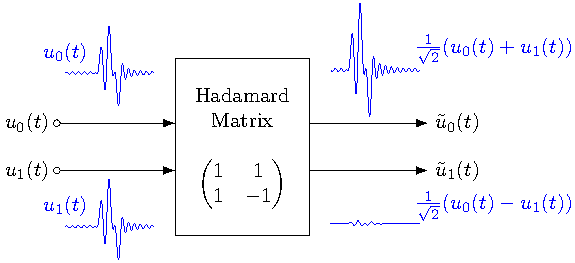
\includegraphics[width=\linewidth]{figures/05hadamard/hadamard_dimension.pdf}
    \caption{An illustration of a pulse arriving at two different receiver elements at the same time. $\utv = \Tr{\left( u_0(t) , u_1(t) \right)}$ is the input signal and $\tilde{\bm{u}}(t) = \Tr{\left( \tilde{u}_0(t) , \tilde{u}_1(t) \right)}$ is the output signal of the Hadamard matrix.}
    \label{fig:hadamard_dimension}
\end{figure}

Any realistic situation would most likely be somewhere in between these two extremes. Whether combining the inputs in a Hadamard ADC gives a direct SNR improvement or not, will depend on which of the two extremes that is closest to the situation at hand. If we denote the output vector of the Hadamard matrix as $\tilde{\bm{u}}(t)$, the analog system will always have to be scaled towards $\E \left[ \norm{\tilde{\bm{u}}(t)}{\infty} \right]$. The question of is wether or not $\E \left[ \norm{\tilde{\bm{u}}(t)}{\infty} \right] < \E \left[ \norm{\utv}{\infty} \right]$.



\subsection{Shared Control Using a Chain-of-Integrators}
In this thesis, the chain of integrators was presented with a local control only, as shown in figure \ref{fig:CI}. It is possible to misalign control and signal dimensions, also for an analog system that integrates the input in a chain structure. The $\Gmat$-matrices could for instance be implemented as Hadamard matrices, hence rotating the control space, even though the states never share the same analog state space. In line with the discussion of section \ref{sec:advanced_DC}, it might also very well be that the Hadamard matrix is not the best choice for these matrices. Due to the orthogonality of the Hadamard transform, it could be considered a general purpose solution. If statistical properties of the input channels is known, this knowledge should be used to find the optimum control mapping.

Applications with signal properties closer to the situation pictured in figure \ref{fig:hadamard_dimension} than that of figure \ref{fig:signal_dimension} are not suited for using the Hadamard analog system. For these applications, combining an integrator chain with a shared digital control would be particularly attractive.






\subsection{Absorbing the LNA Into the ADC}
Systems receiving weak analog information signals, often use a low noise amplifier (LNA) to amplify the signal before A/D conversion. When using a control-bounded converter, there should ideally not be any components before the ADC. The overall system performance achievable by including an LNA into the ADC, versus keeping it on the outside, is not evaluated. However, it would be a surprising result if separating the two components showed to be the most attractive. We propose as a general rule of thumb, that one should aim to include as much of the necessary functionality into the ADC as possible, as this will most likely reduce the requirements on the involved components. However, the associated design complexity and necessary implementation time must also be considered in the trade-off.

In the presented work, the control gain $\kappa$ is not given much attention. In an application that normally uses an LNA, absorbing it into the ADC would give the ADC a much weaker input signal. This is prior knowledge of $b_{\bm{u}}$ that should be utilized. In this case, the control gain $\kappa$ should probably not be equal for all control signals. In an integrator chain for instance, the first integrator will have a weak input signal. Hence, this integrator could have been stabilized with less control gain, which in turn allows a higher $\beta$. This scaling would give a direct performance increasement, cf. (\ref{eq:analytic_snr_est}).





\subsection{Comparator Offset Voltage}
Another advantage of control-bounded ADCs that should be mentioned, is the sensitivity to offset voltage in the comparators. As highlighted several times, the only information about the control signals that is used by the digital estimator is that this was the signal needed to stabilize the internal states of the analog system. The digital estimator do not care about how these control signals relate to the input or the states of the analog system. Note that $\Gmattilde$ is not used by the digital estimator in figure \ref{fig:de_problem}. This means that the output estimate is completely invariant to the offset voltage of the comparators, as long as the offset voltage is not disabling the digital control from bounding the state vector.

Figure \ref{fig:offset_sim} verifies this statement. The figure shows the PSD of the estimated input signal, $\utvhat$, from a chain-of-integrator simulation where the input referred offset voltage of the comparators is varied. The parameters used for the simulation is identical to that of table \ref{tab:CI_params}. In particular, the supply voltage used is $\SI{1}{\volt}$. The input referred offset voltage is modelled by adjusting the reference voltage of the ideal comparators. The reference voltage is varied from 0 to $\SI{700}{\milli\volt}$.

The key point of the figure is to show that an offset voltage of $\SI{300}{\milli\volt}$ has essentially no effect on the output estimate. When the offset voltage is increased to $\SI{500}{\milli\volt}$ and $\SI{700}{\milli\volt}$, the digital control is no longer able to properly bound the state vector and the quality of the estimate is reduced.

\begin{figure}[htbp]
    \centering
    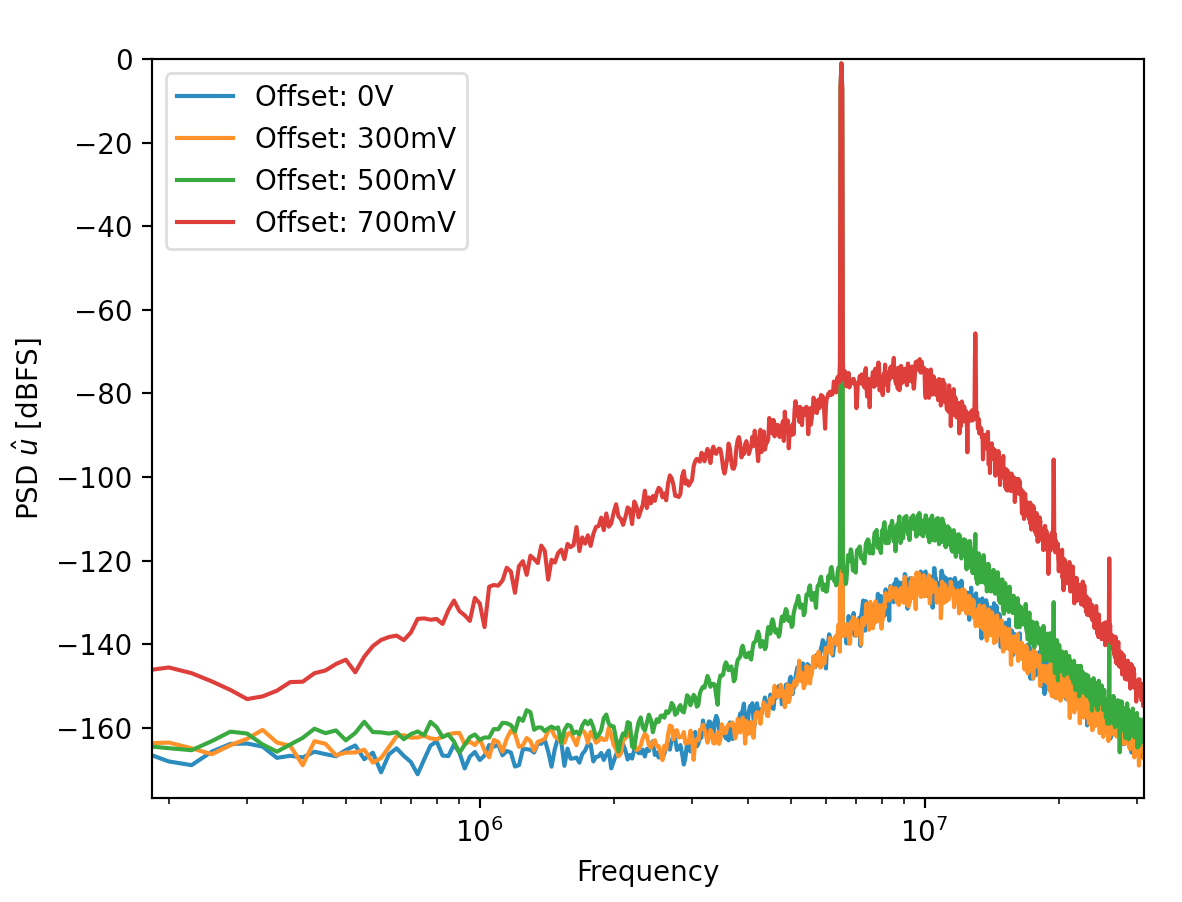
\includegraphics[width=\linewidth]{figures/060discussion/offset_sim.png}
    \caption{PSD of $\utvhat$ from a chain-of-integrator simulation, where the input offset voltage of the comparators is varied. The simulated circuit has a supply voltage of $\SI{1}{\volt}$ and the input offset voltage of the comparators are varied between 0 and $\SI{700}{\milli\volt}$ as indicated.}
    \label{fig:offset_sim}
\end{figure}





\subsection{Noise in the Hadamard System}
An important non-ideality that is not treated in this thesis is the noise generated by the components of the analog system. When the signal is integrated in a chain structure, the first integrator will be the most critical and most of the power budget will be consumed by this integrator in order to keep its noise contribution according to the requirement. In the Hadamard ADC however, all integrators in the first column will contribute equally to the total output noise. It was shown in \cite{malmberg_thesis} that it is possible tune the situation by amplifying the different signal dimensions unequally. By increasing the gain of one/some signal dimensions, and reducing it on others, the noise contribution is distributed unequally between the integrators. This however comes at an expense of reduced nominal performance.

The input node of the system is critical, as this is where the information carrying input signal is at its weakest. The vulnerable input signal should be handled with care, and connecting more active components to this node does not intuitively sound beneficial. However, when designing the active components, trade-offs will have to be made between noise, speed, linearity, etc., and other design specification might influence the cost of reaching a certain noise requirement. A thorough noise analysis of the different architectures remains for future work.
















\section{Limitations of the Presented Work}
Some limitations of the presented work is discussed in this section.


\subsection{Filter Complexity}
The work of this thesis is mainly concerned with the analog system and the digital control of the proposed architecture. The simulations are performed using an offline estimation filter implemented in Python. An efficient, online filter algorithm is presented in \cite{malmberg_thesis}, but is not tested in this work. The power consumed by the estimation filter will of course count on the total power budget of the ADC, and should therefore be taken into account when evaluating the overall system performance.

For larger systems with several input channels, it might be more efficient to run the algorithm on a micro-controller, rather than using a dedicated HDL implementation of the filter algorithm. These are interesting questions that remains for future research.


\subsection{Complex Poles and Optimized Transfer Function}
In this thesis, the analog transfer function of both the chain-of-integrators and the Hadamard system constitutes a chain of first order integrations. However, in a practical realization it would be favorable to have more advanced transfer functions in the analog system. Adding zeros in the transfer function enables band-pass and notch filter realizations, and complex pole pairs enables sharper transitions between pass-band and stop-band. This way, more of the analog system gain may be concentrated in the frequency band of interest, resulting in an overall performance increasement. Optimizing the noise transfer function is an important part of the design of $\sd$ modulators and should be done in control-bounded ADCs as well.

It was shown in \cite{malmberg_thesis} how a chain-of-integrator-like structure can be modified to allow for any general $N$-th order transfer function polynomial. Poles are introduces to the transfer function by connecting the different states through additional feedback loops, and zeros by feed-forward paths from the input. The same general transfer function is also achievable for the Hadamard system by using a similar structure.

Evaluating the proposed architecture with an optimized transfer function is unfortunately beyond the scope of this thesis. The main focus has been to find and evaluate an efficient realization of the Hadamard analog system, and optimized transfer functions is kept in mind as an important part of future development.



\subsection{Quantitative Measures}
The simulations presented in this thesis are only meant to give a qualitative indication of the performance of the different architectures. When designing for a specific application one would want to find the optimum filter order, OSR, integrator gain, state boundary etc., in order to reach the performance requirements with the lowest possible power consumption.

The simulations performed in this thesis are highly ideal, and no attempt has been made to do such optimizations. These optimizations will be considered together with transistor level implementations in the given technology and the goal of this thesis is to provide a useful background for the next part of the design process.



